%
%----------------------------------------------------------------------------------------
%	PACKAGES AND DOCUMENT CONFIGURATIONS
%----------------------------------------------------------------------------------------
%

\documentclass[12pt]{article} %report, article, amsart, exam
\usepackage[letterpaper,margin=1in]{geometry}
\usepackage{fancyhdr,color}
\usepackage{tikz,graphicx,multicol}
\usepackage{amssymb,euscript,eufrak,nicefrac,enumitem}
\usepackage{amsfonts,amsmath,amsthm} %don't need with 'amsart' document class
\usepackage{hyperref}
\usepackage{comment}
\usepackage{scrextend} %needed for addmargin environment
\usepackage{graphicx} 
\usepackage{listings}

\usepackage{color}
\usepackage{accsupp}
\usepackage{booktabs}
\usepackage{subcaption}

\definecolor{dkblue}{rgb}{0,0,0.5}
\definecolor{comment}{rgb}{1,0,0}
\definecolor{mauve}{rgb}{.627,.126,.941}
\definecolor{purple}{rgb}{0.5, 0, 0.545098}

\lstdefinestyle{customc}{
  belowcaptionskip=1\baselineskip,
  breaklines=true,
  frame=L,
  xleftmargin=\parindent,
  language=C,
  showstringspaces=false,
  basicstyle=\footnotesize\ttfamily,
  keywordstyle=\bfseries\color{green!40!black},
  commentstyle=\itshape\color{purple!40!black},
  identifierstyle=\color{blue},
  stringstyle=\color{orange},
}

\lstdefinestyle{customasm}{
  belowcaptionskip=1\baselineskip,
  frame=L,
  xleftmargin=\parindent,
  language=[x86masm]Assembler,
  basicstyle=\footnotesize\ttfamily,
  commentstyle=\itshape\color{purple!40!black},
}

\lstset{escapechar=@,style=customc}

%
%----------------------------------------------------------------------------------------
%% Define headers & footers
%----------------------------------------------------------------------------------------

\pagestyle{fancy}
   \lhead{} 
   %\chead{Loyola University Chicago} 
   \rhead{}
   \renewcommand{\headrulewidth}{0pt}
   \addtolength{\footnotesep}{5mm}
 
%
%----------------------------------------------------------------------------------------
%% Some user-defined colors
%----------------------------------------------------------------

\setlength{\parskip}{1em}
\renewcommand{\baselinestretch}{1.3}

%
%----------------------------------------------------------------------------------------
%% BEGIN: topmatter
%----------------------------------------------------------------------------------------
%

\title{ COMP 464 - High Performance Computing \\ Distributed memory N-body with MPI} % Title
\author{
Loyola University Chicago \\
Jose Luis Rodriguez 
} % Author name
\date{\today} % Date for the report

%
%% END: topmatter
%%------------------------------

\begin{document}

\maketitle

\thispagestyle{fancy}

%---------------------------------------------------------------------------------------- 
%	SECTION 1 - PROBLEM STATEMENT
%----------------------------------------------------------------------------------------

\section{Overview}

This report highlights the procedures and results of running an mpi program (mpi\_nbody3.cpp) that predicts the individual motion of a group of celestial objects (particles) interacting with each other gravitationally. The program also runs a series of experiments and generates a benchmark (max, min and average speed of particles) as well as other metrics to evaluate the performance of the program. 

This code is execute on The University of Texas at Austin Texas Advanced Computing Center (TACC) Stampede2. The mpi\_nbody3 code was compile using the Intel C++ compiler (icpc) and the openMPI library in order to parallelize the serial code details and specifications to follow.

The n-body problem code performs two major benchmarks in order to compute strong scalability and weak scalability. The program was compiled in serial and parallel each version was tested with 1,000, 2,000, 4,000, and 8,000 particles and 1, 2, 4, 8, 16, 32, 64, 128 and 256 ranks across 4 different nodes and the same number of steps (-s 100) and for weak scaling the number of particles was increased proportionally to the number of ranks. 

\section{Benchmark Analysis}

\textbf{Code Modifications} 

 The average time per number of particles was recored in order to compute the strong scalability as well as the ranks time standard deviation. By keeping a constant workload per-rank it is possible the code weak scale efficiency as we are keeping a constant workload per-thread when the number of particles increase the number of threads also increased. In order to perform the benchmarks in parallel, a series of changes to the code were necessary in order to initialize it to work with openMPI commands to parallelize sections if the code such as the loop use on the accelerate, update and search functions. MPI allows to perform parallel computations by running a copy of the code in each rank, hence it is necessary to identify a root rank to write and display output correctly. 

Besides the root rank it is necessary to plan how to gather the data in each rank or how to propagate the data to other nodes in order to perform different operation utilizing the information in each rank the later. The passing of messages and information between MPI ranks creates an overhead measured in the benchmarks as well as the ranks time standard deviation for the different particle sizes. Now when comparing OpenMPI scalability with OpenMP from the benchmark perspective they two behave similarly as both speedup goes up as the number of ranks goes up and efficiency decreases as the number of ranks increases proportionally to the number of particles.  

Now when looking at the actual time that it took to run the different benchmarks then we see that the OpenMPI code perform significantly slower than the OpenMP implementation. As to perform the calculation on the benchmarks ranks need to communicate (broadcast) the results of their calculations so all ranks have the same data available global calculation are necessary to perform. It is interesting to see how in the strong scaling case as number of ranks increases the ratio between the MPI commands and the global time increased. Different from the weak scaling where are the number of particles increase proportionally to number of particles the ratio is much lower.

\subsection{Strong scalability}

When computing the strong scalability for the nbody problem the particles size stays fixed while the number of threads increase. In Figure.1 this benchmark was perform on 1000, 2000, 4000, 8000 and 16000 particles and for each set of particles the benchmark was run with 1, 2, 4, $\dots$ 256 ranks and 1000, 2000, 4000, 8000 and 16000 particles. We can see in the chart how the nbody problem follows shows the strong scalability principle as its almost a perfect speedup ( execution time goes down with the number of threads). We can see how when using a relative small number of particles as the ranks increased the overhead of the communication between different ranks affects performance.

Finally for the deviation of the time when the number of ranks the number of particles is smaller there is a greater deviation in running time of the code, it settles for some higher number of particles, both cases strong and weak scaling show similar behavior although the standard deviation for larger values in the weak scaling benchmarks has less deviation.

\begin{figure}[htb]
\caption{Strong Scaling - Speed-Up (T1/Tp)}\label{fig:benchmark01}
\centering
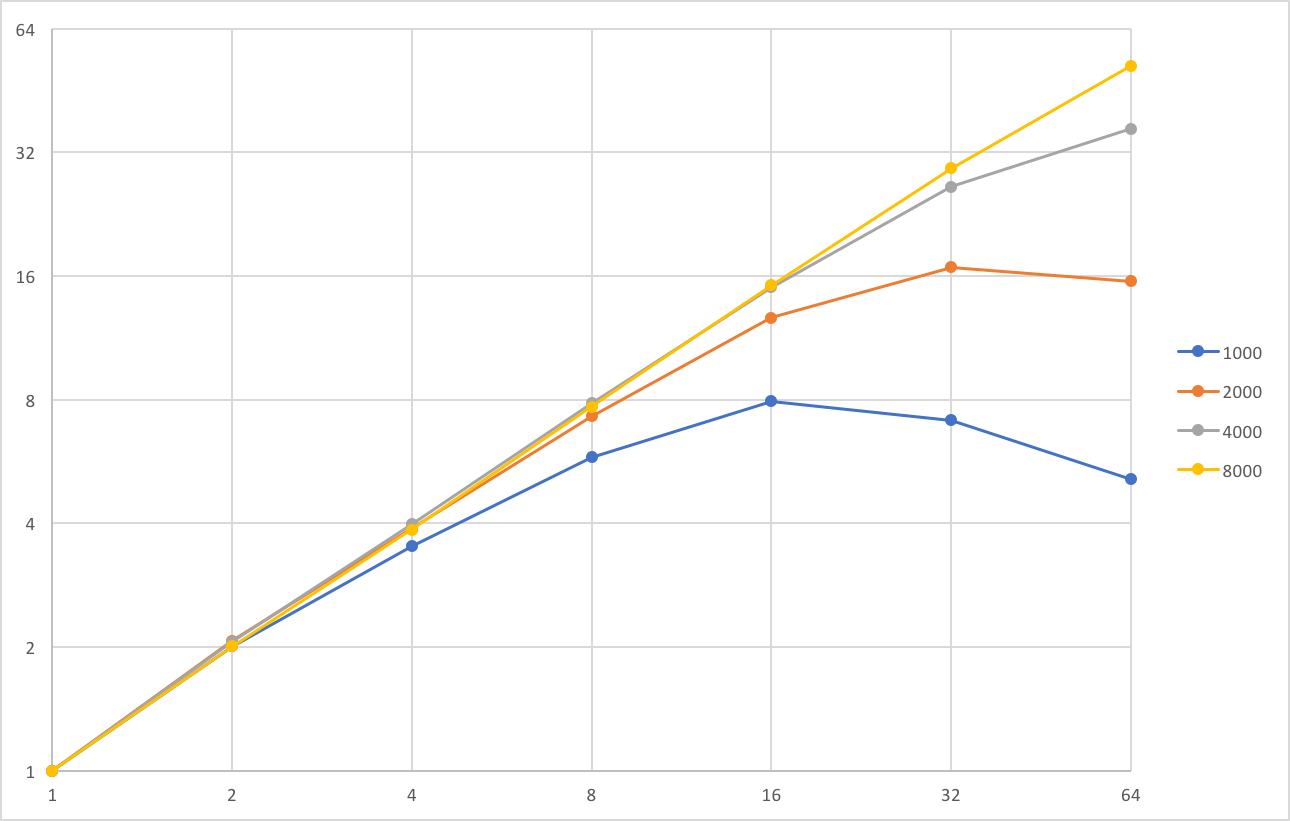
\includegraphics[width=15cm,keepaspectratio]{imgs/img01.png}
\end{figure} 

\newpage

The other measure to identify how far the nbody problem is from the ideal speed we compute the efficient. In Figure.2 we can see how as the number of ranks increases depending of the particles sized the efficiency of the parallel program decreased. 

This is due to that in many cases starting the communication between the different ranks creates decreasing performance of program. This is due that when there are more ranks than particles (problem size not scale proportionally to the number of ranks) the program efficiency will decrease significantly as number of ranks increase. Hence in this case having more ranks it doesnt translate to better performance.

\begin{figure}[htb]
\caption{Strong Scaling - Efficiency (Sp/P)}\label{fig:benchmark01}
\centering
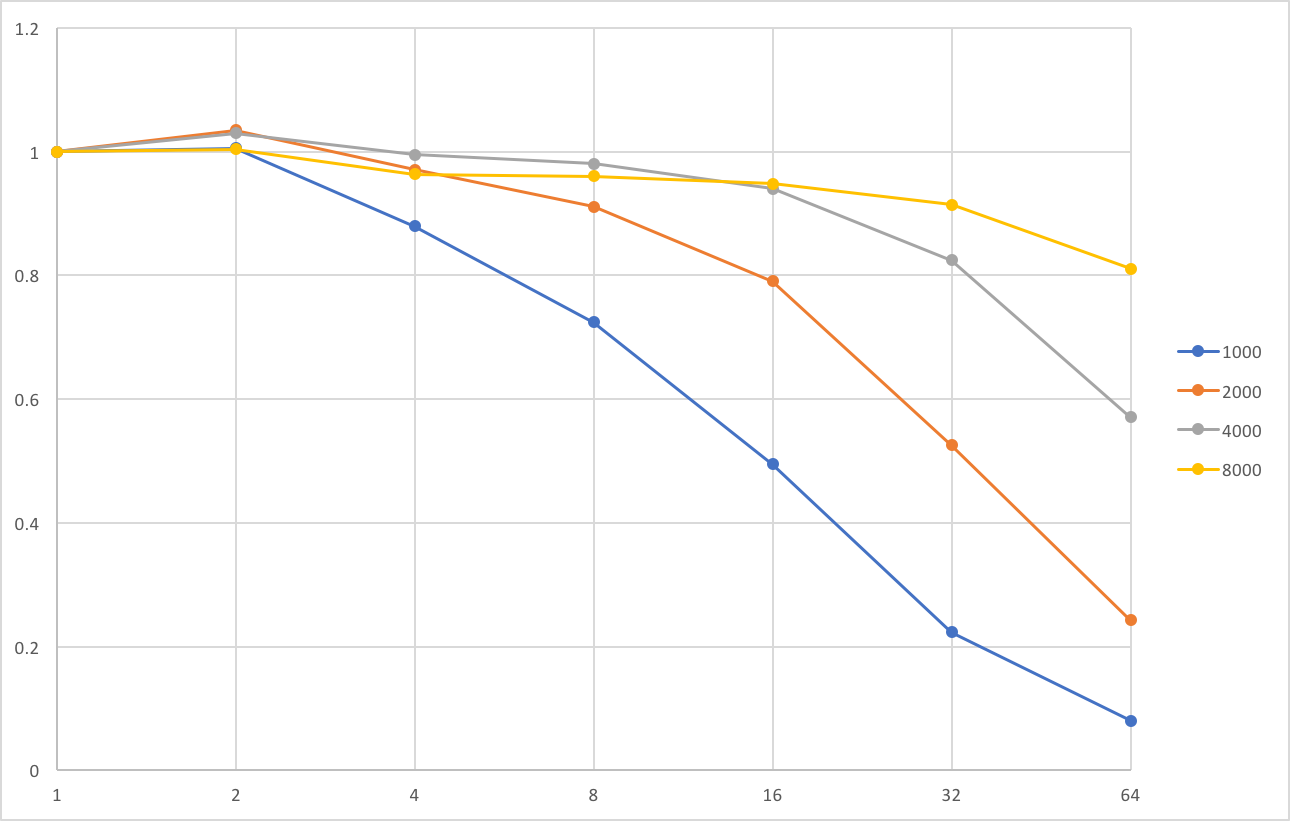
\includegraphics[width=\textwidth,keepaspectratio]{imgs/img02.png}
\end{figure} 

\newpage

\subsection{Weak scalability}

A more realistic accurate way to measure the efficiency of a parallel program is by distributing data in this case particles amount all ranks evenly in order to avoid idling due to some threads having less data to process. To summarize as the number of ranks increase the number of particles should increase proportionally as it will allow to compensate for the communication overhead part of openMPI when ranks have to share data to perform operations. In some cases when the data is not distributed evenly between all the ranks then it is possible to encounter errors as miscalculations as all ranks should work on similar size data. 

These are some of the reason why the actual speedup and efficiency decreased when running the strong scaling benchmarks. For the case of weak scalability on the nbody problem as the particles and threads increase we want to keep the amount of data per thread to stay constant or as close to constant as possible to achieve constant execution time. For the case of weak scalability efficiency in Figure.4 the numbers of particles are given by the recursive function $ P_i = \sqrt{2} \times P_{i-1} $. We can see how as the number of particles and threads increase efficiency also increases.

\begin{figure}[htb]
\caption{Weak Scaling - Efficiency ($T_1/T_p$)}\label{fig:benchmark02}
\centering
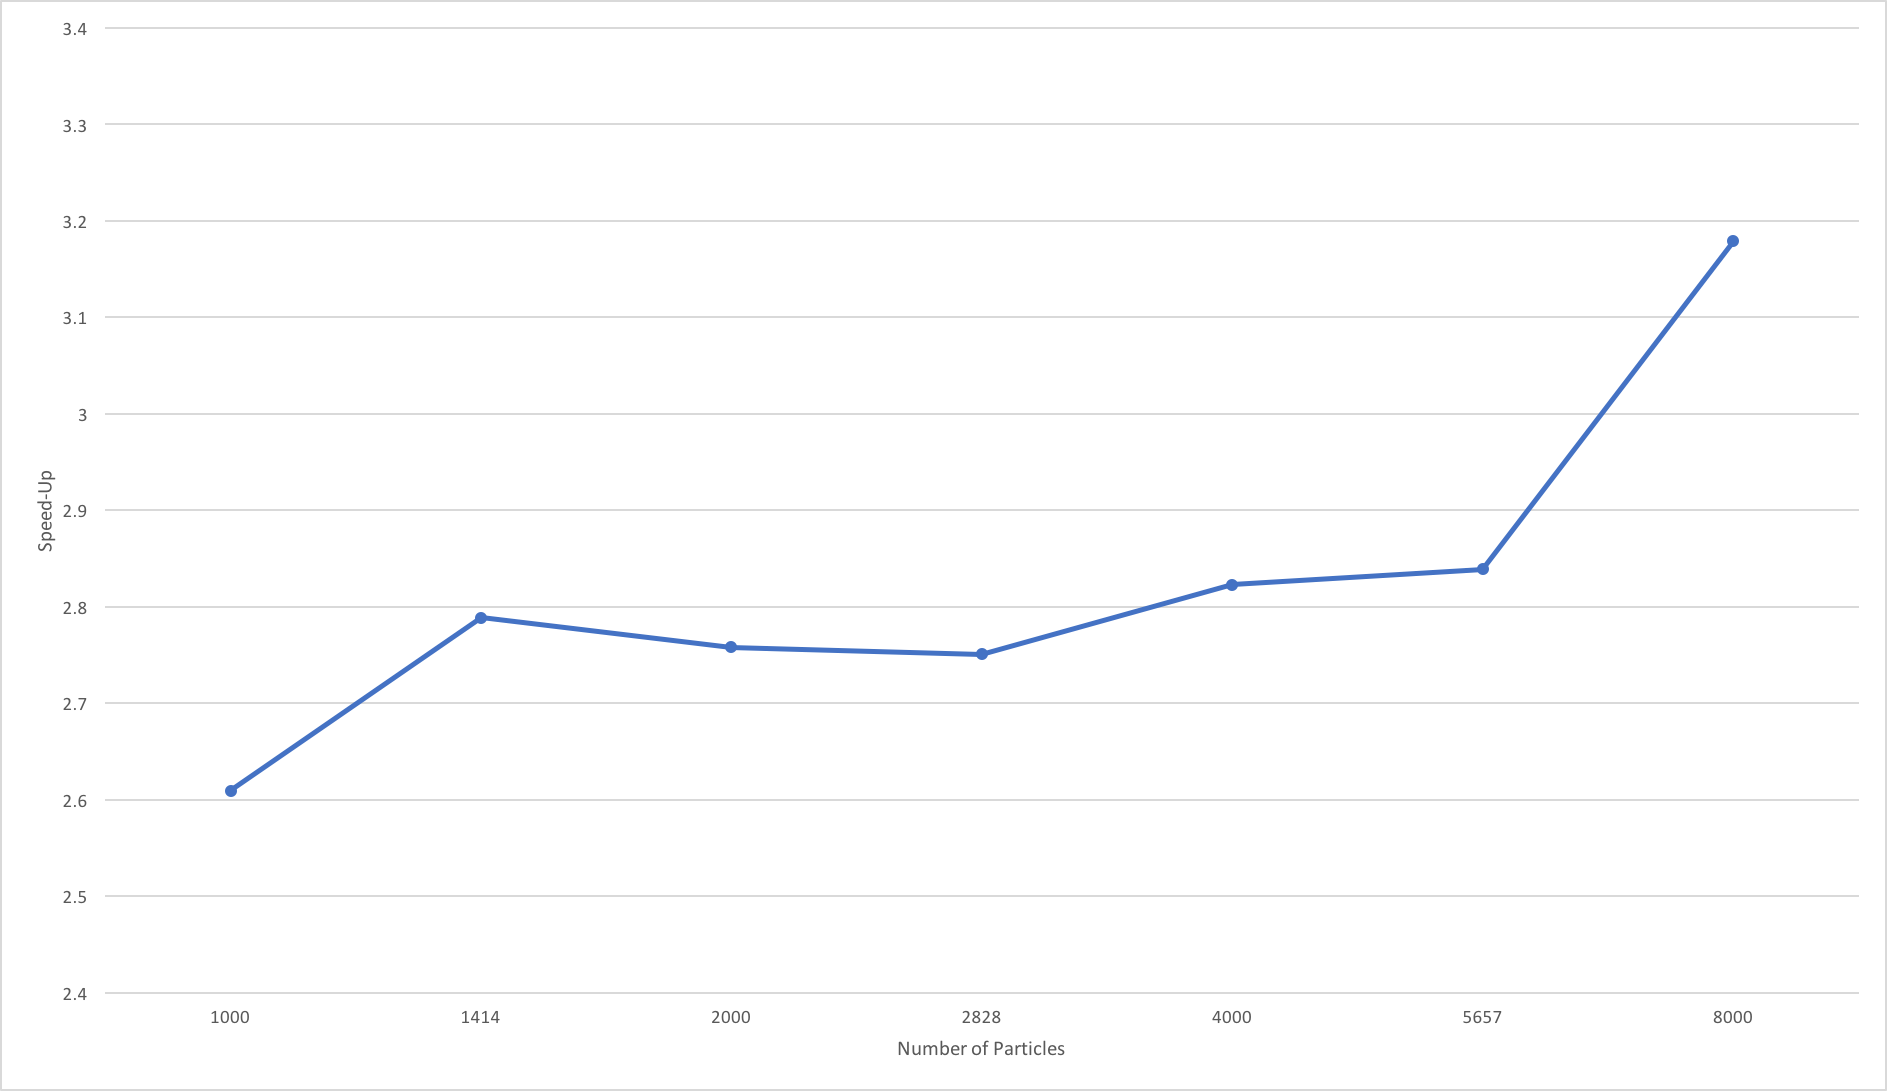
\includegraphics[width=\textwidth,keepaspectratio]{imgs/img03.png}
\end{figure}

\section{Running Time Benchmarks}

\subsection{Strong Scaling Runtime}

Due to nature of OpenMPI (send, receive messages), it is possible determine the time that takes for an MPI command to send/receive messages and the time spent in the library functions. By doing this we will determine the added overhead to the code. In Figure.4 we can see how as the number of ranks increases depending of the particles sized the time spend sending/receiving messages increased, this is the overhead added by  spreading the problem in different ranks.

\begin{figure}[htb]
\caption{Communication Runtime - Strong Scaling}\label{fig:benchmark05}
\centering
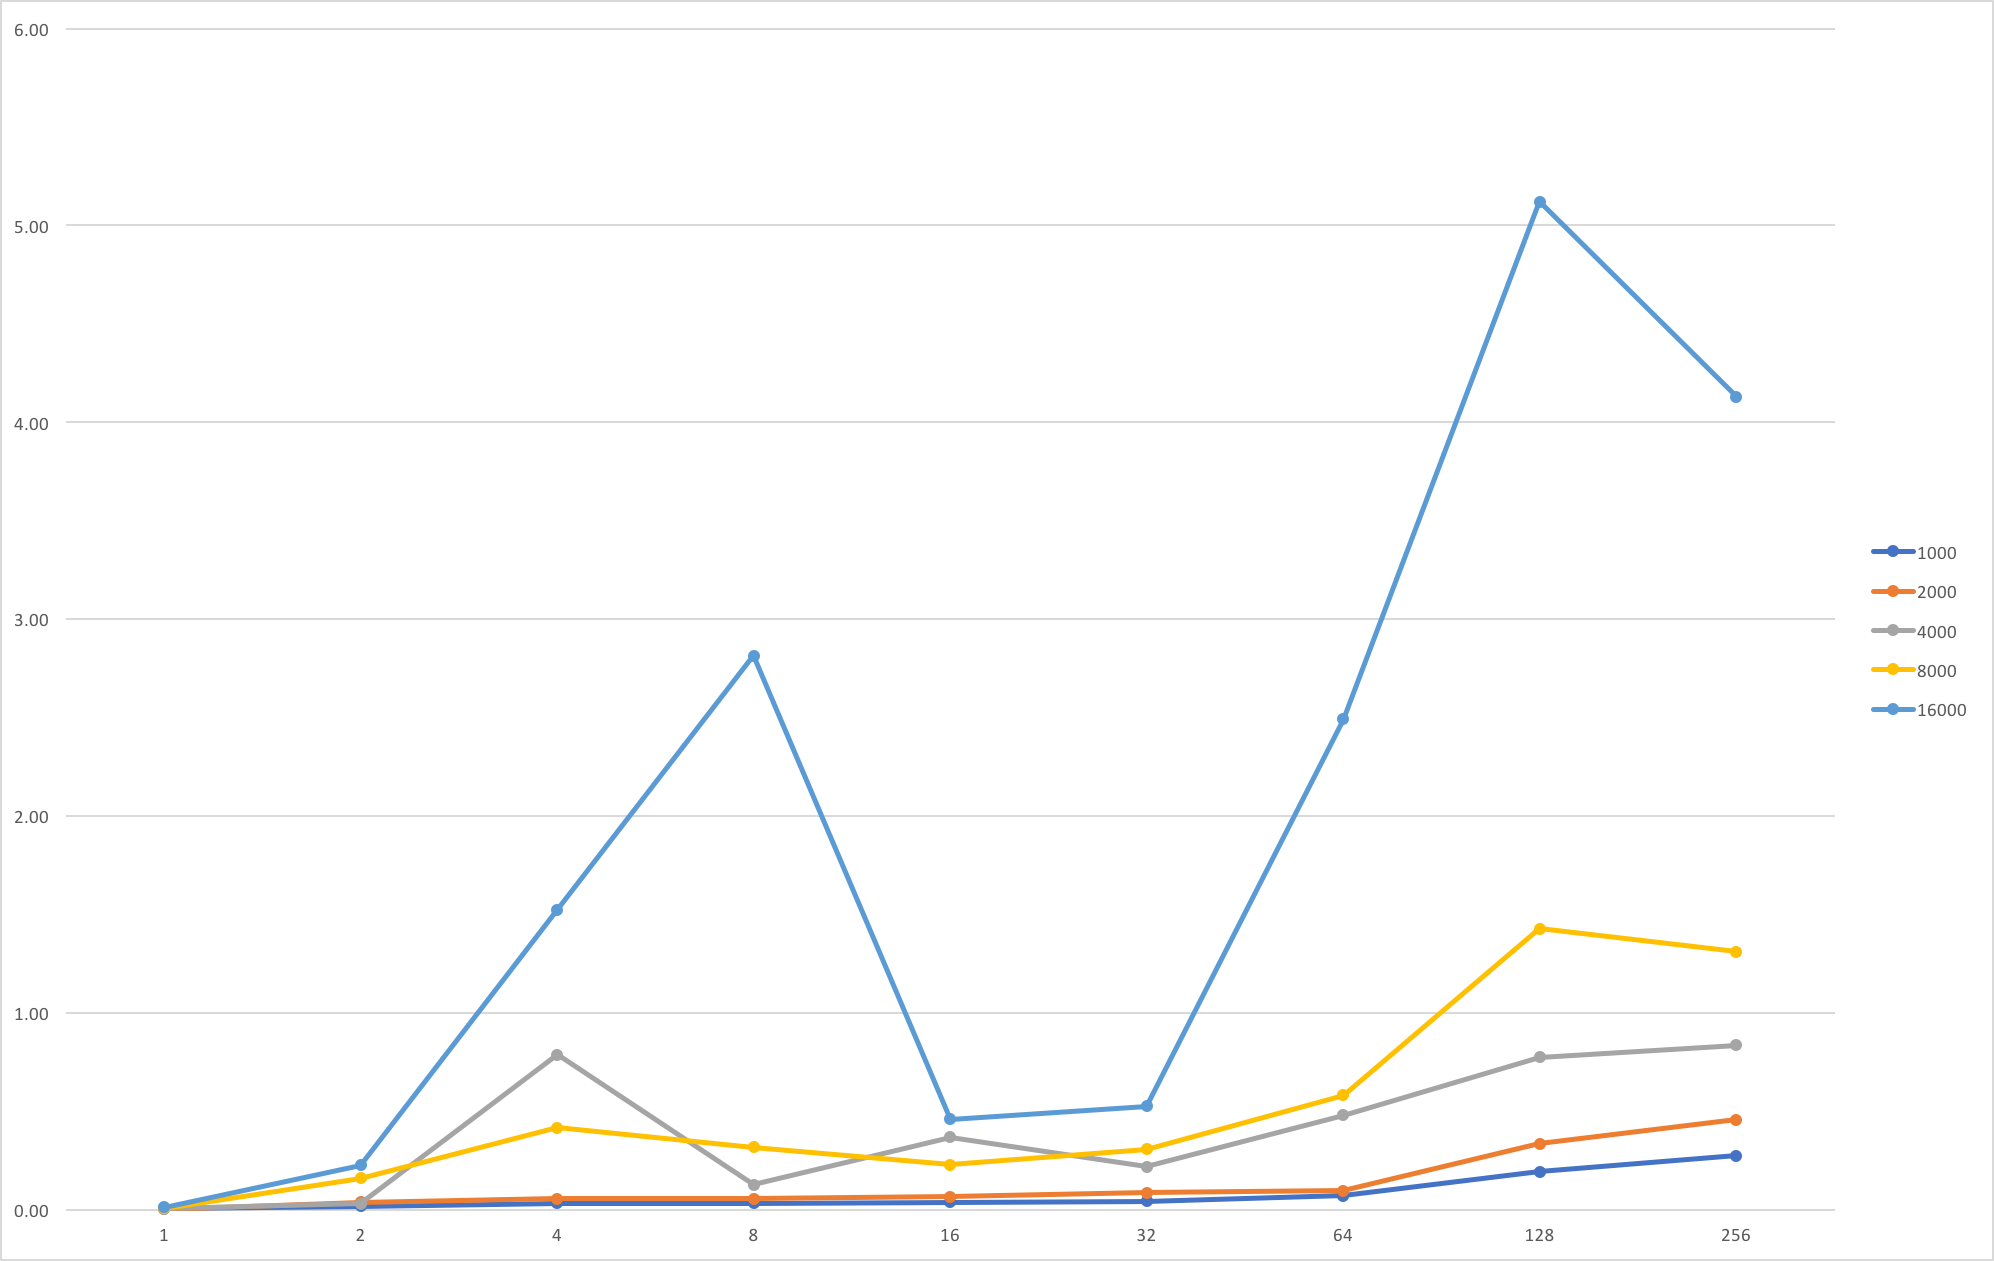
\includegraphics[width=\textwidth,keepaspectratio]{imgs/img04.png}
\end{figure}

\newpage

As the number of ranks increases the ratio between the MPI communication framework runtime and the total time increases. Indicating how much is spent sending/receiving messages in MPI library and the rest of the code.

\begin{figure}[ht]
\caption{Ratio Communication Runtime to Total Time - Strong Scaling}\label{fig:benchmark05}
\centering
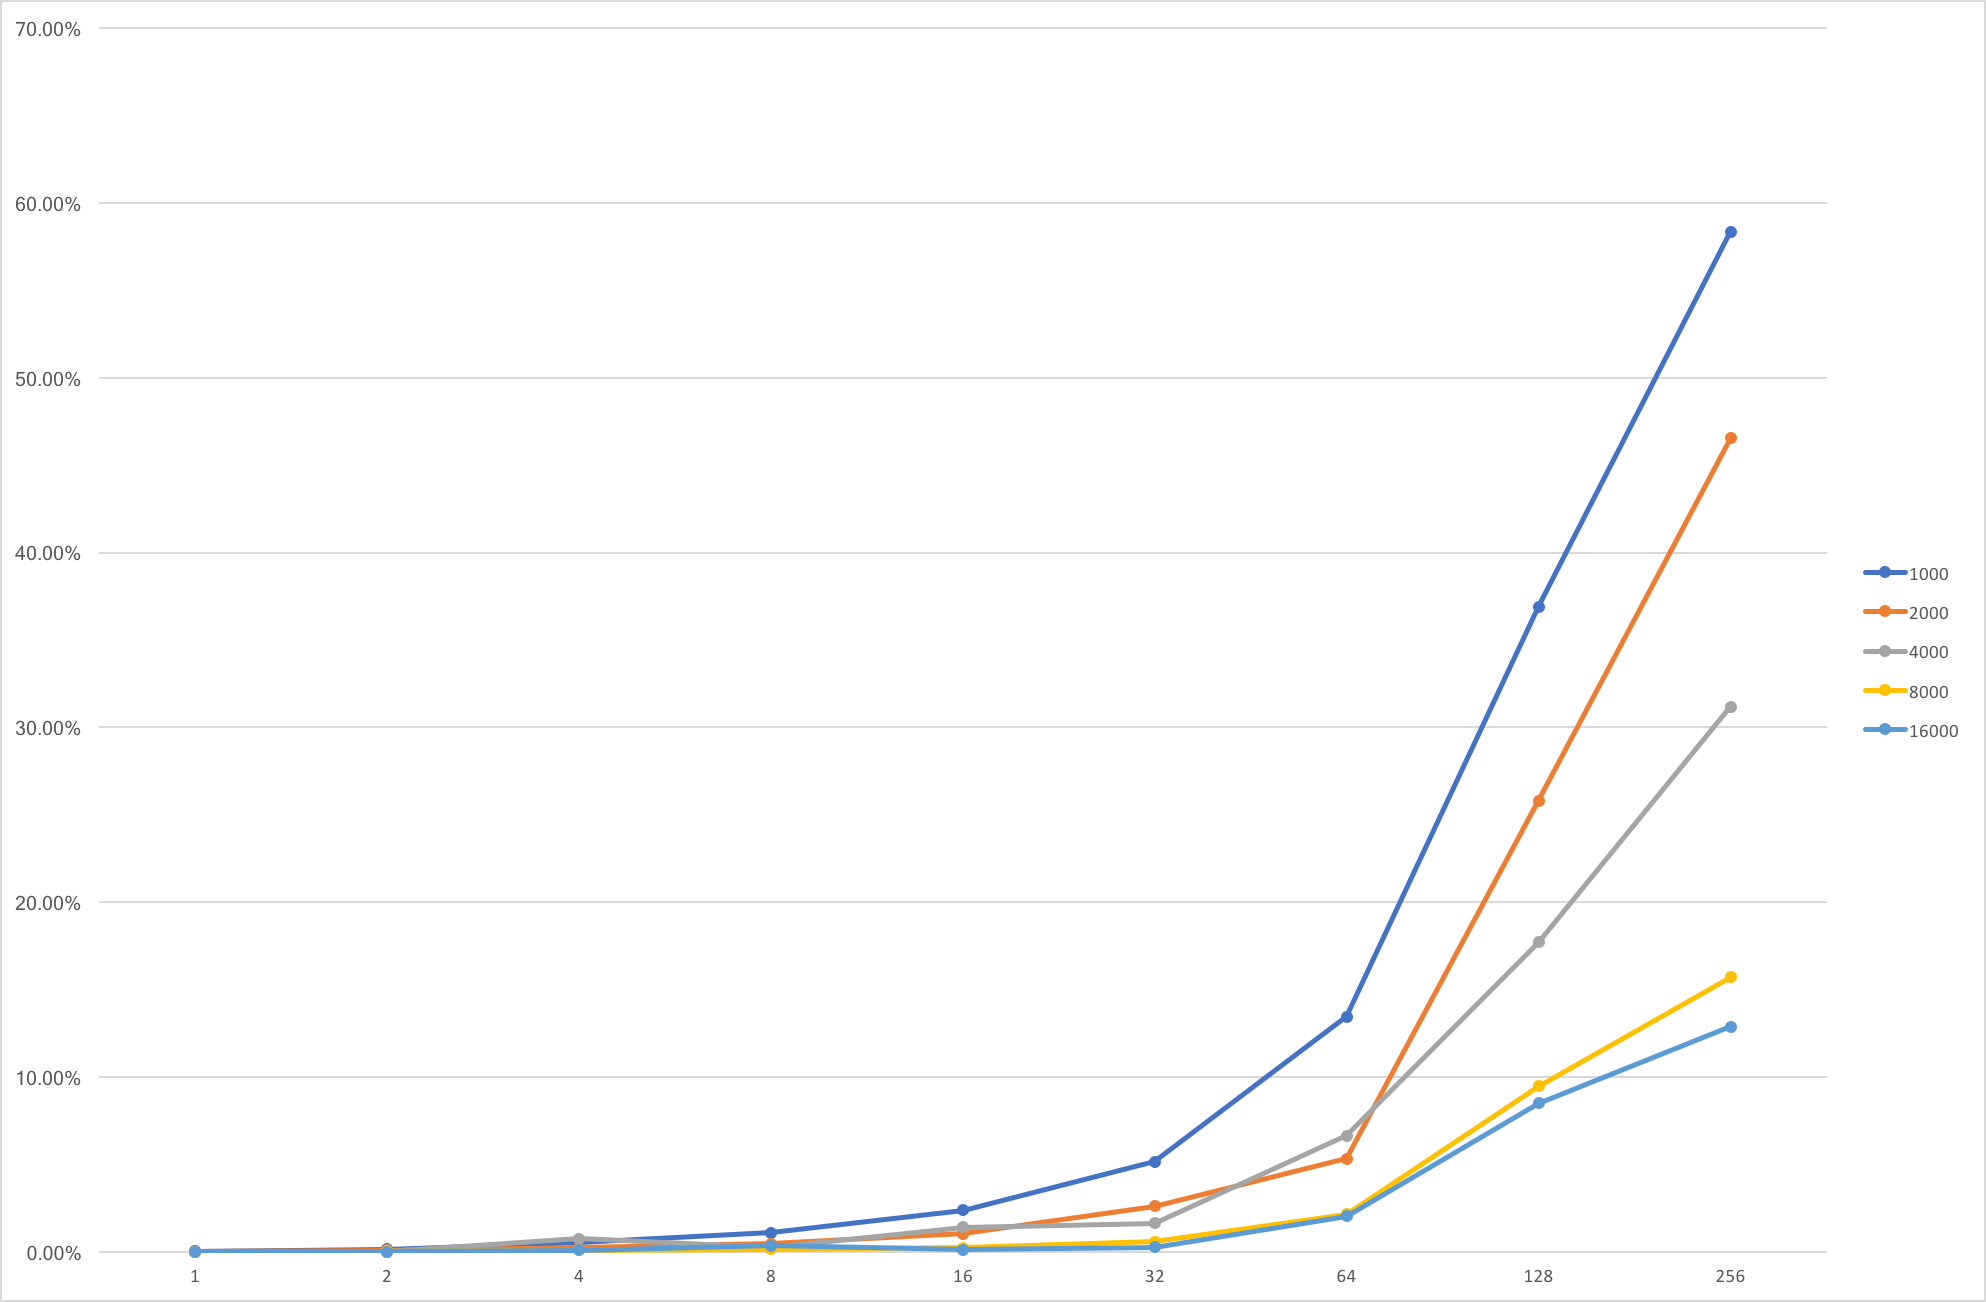
\includegraphics[width=\textwidth,keepaspectratio]{imgs/img05.png}
\end{figure}

\newpage

It is also interesting to explore the time deviation between all the nodes and the over all running time. In Figure.6 we can see that as the number of ranks increases the standard deviation for four and sixteen ranks increases.

\begin{figure}[htb]
\caption{Time Standard Deviation - Ranks 2 to 16 }\label{fig:benchmark05}
\centering
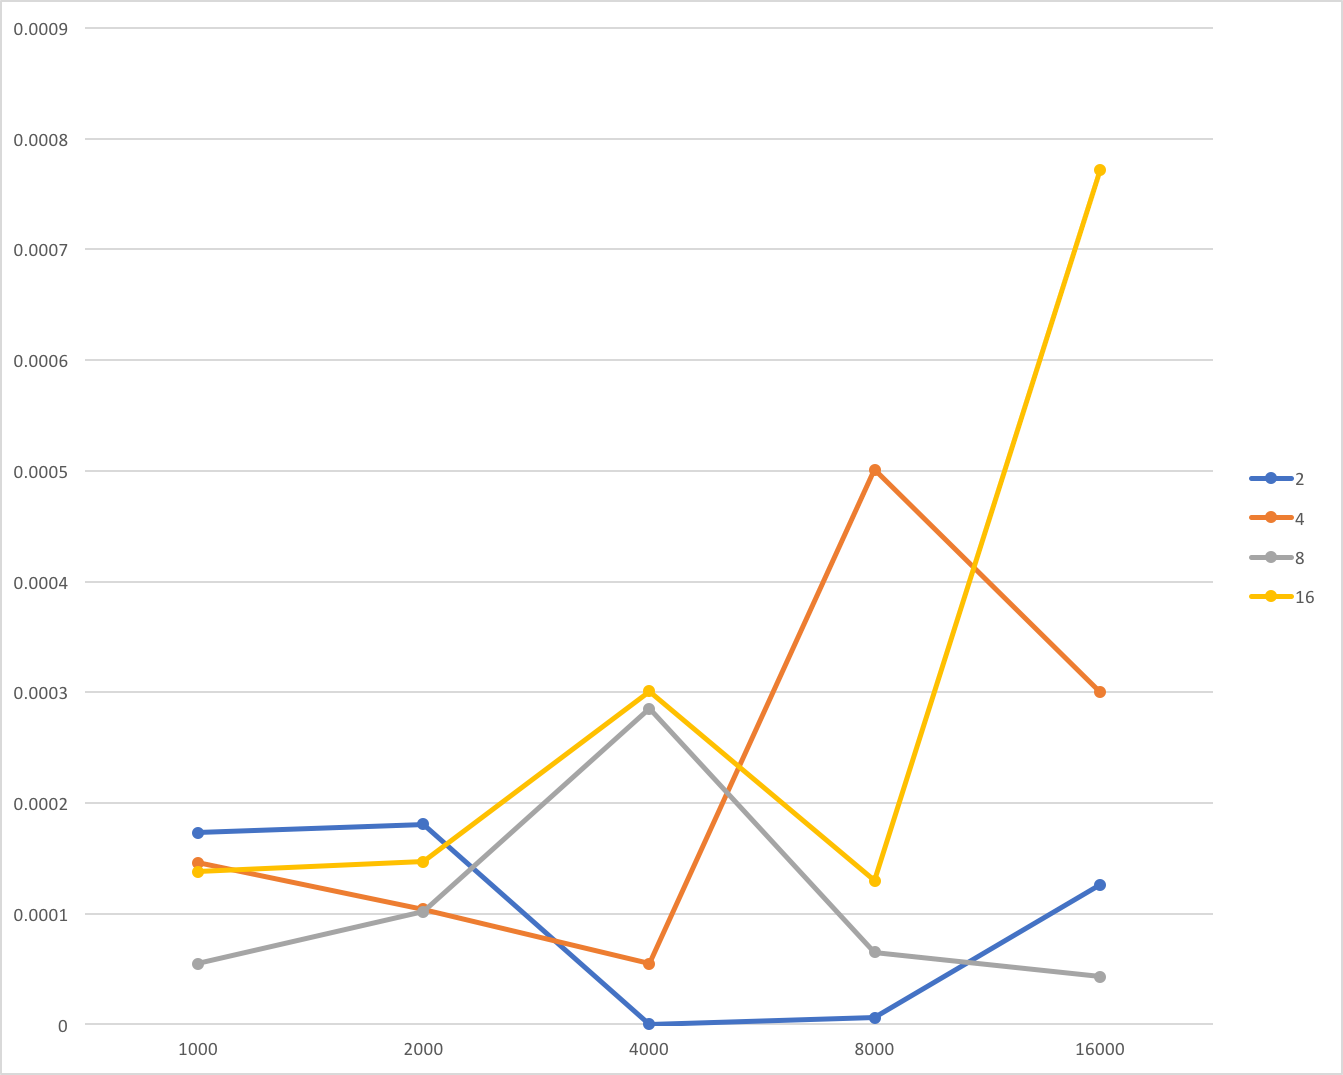
\includegraphics[width=\textwidth,keepaspectratio]{imgs/img08.png}
\end{figure}

\newpage

Now when the number of ranks is higher there is not as much variation on the time spend sending/receiving messages in the MPI library. 

\begin{figure}[htb]
\caption{Time Standard Deviation - Ranks 32 to 256}\label{fig:benchmark05}
\centering
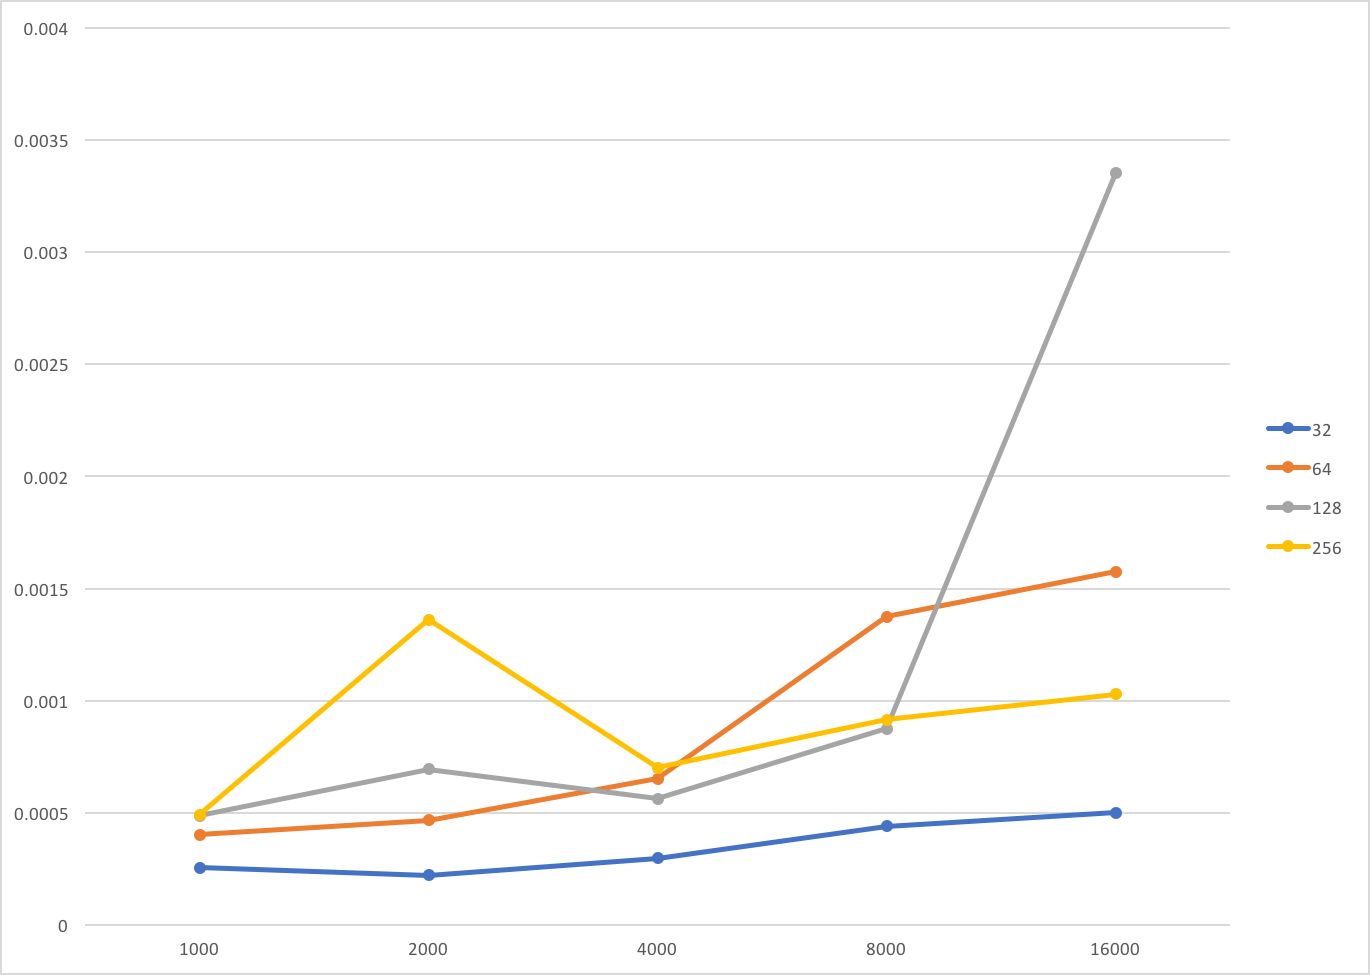
\includegraphics[width=\textwidth,keepaspectratio]{imgs/img09.png}
\end{figure}

\newpage

\subsection{Weak Scaling Runtime}

In Figure.8 there is an interesting spike of time spend in the MPI library when the number of particles is 2828 but more or less it behaves similarly to the strong scalability benchmark by keeping the number of particles relative to the number of ranks the time spend on the MPI library is more or less constant for a given number of ranks.

\begin{figure}[htb]
\caption{Communication Runtime - Weak Scaling}\label{fig:benchmark05}
\centering
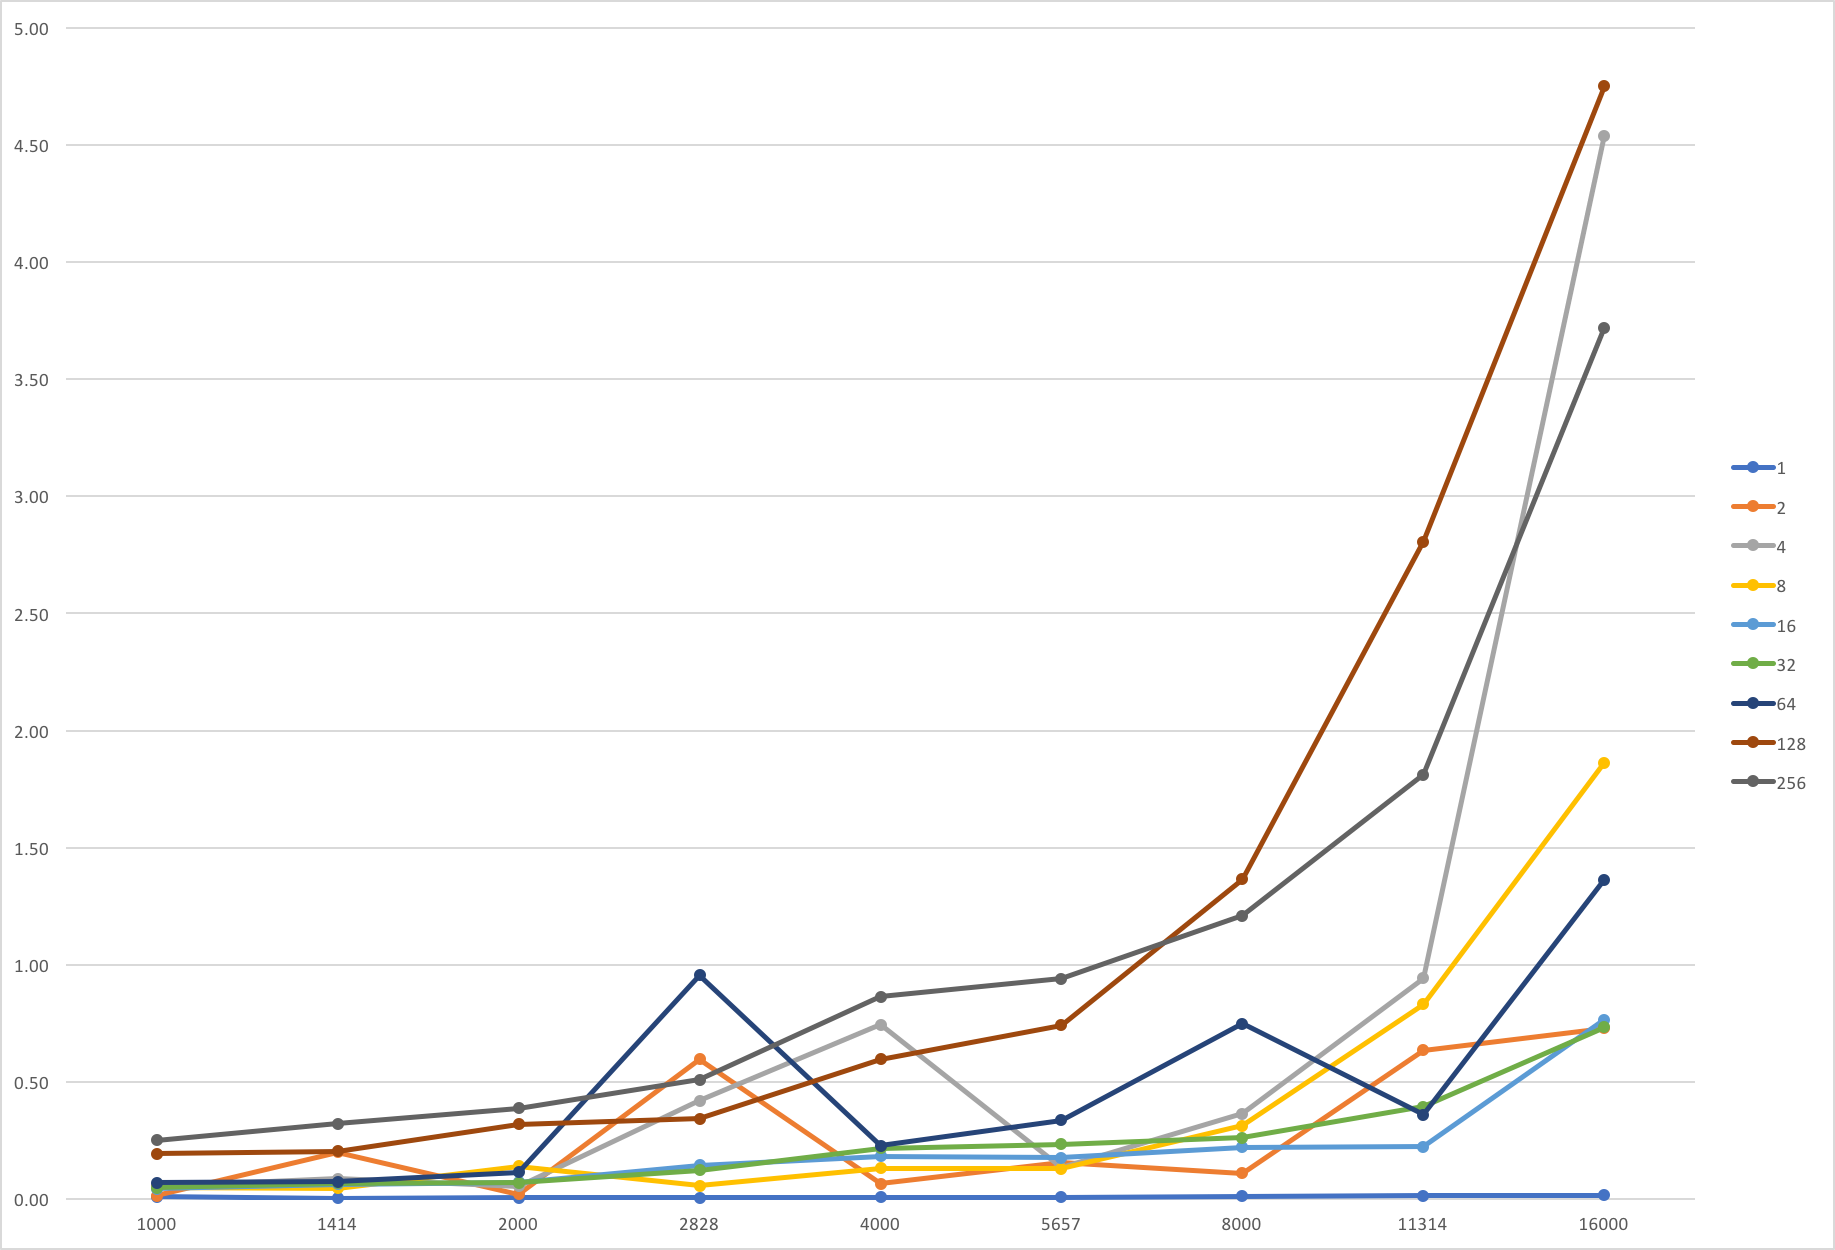
\includegraphics[width=\textwidth,keepaspectratio]{imgs/img06.png}
\end{figure}

\newpage

For the ratio between the communication MPI library time and the overall time that took to execute the code. In Figure.9 we can see how if the number of particles is increased proportionally to the number of ranks then it is possible to decrease the overall time spend in the MPI library.

\begin{figure}[htb]
\caption{Ratio Communication Runtime to Total Time - Weak Scaling}\label{fig:benchmark05}
\centering
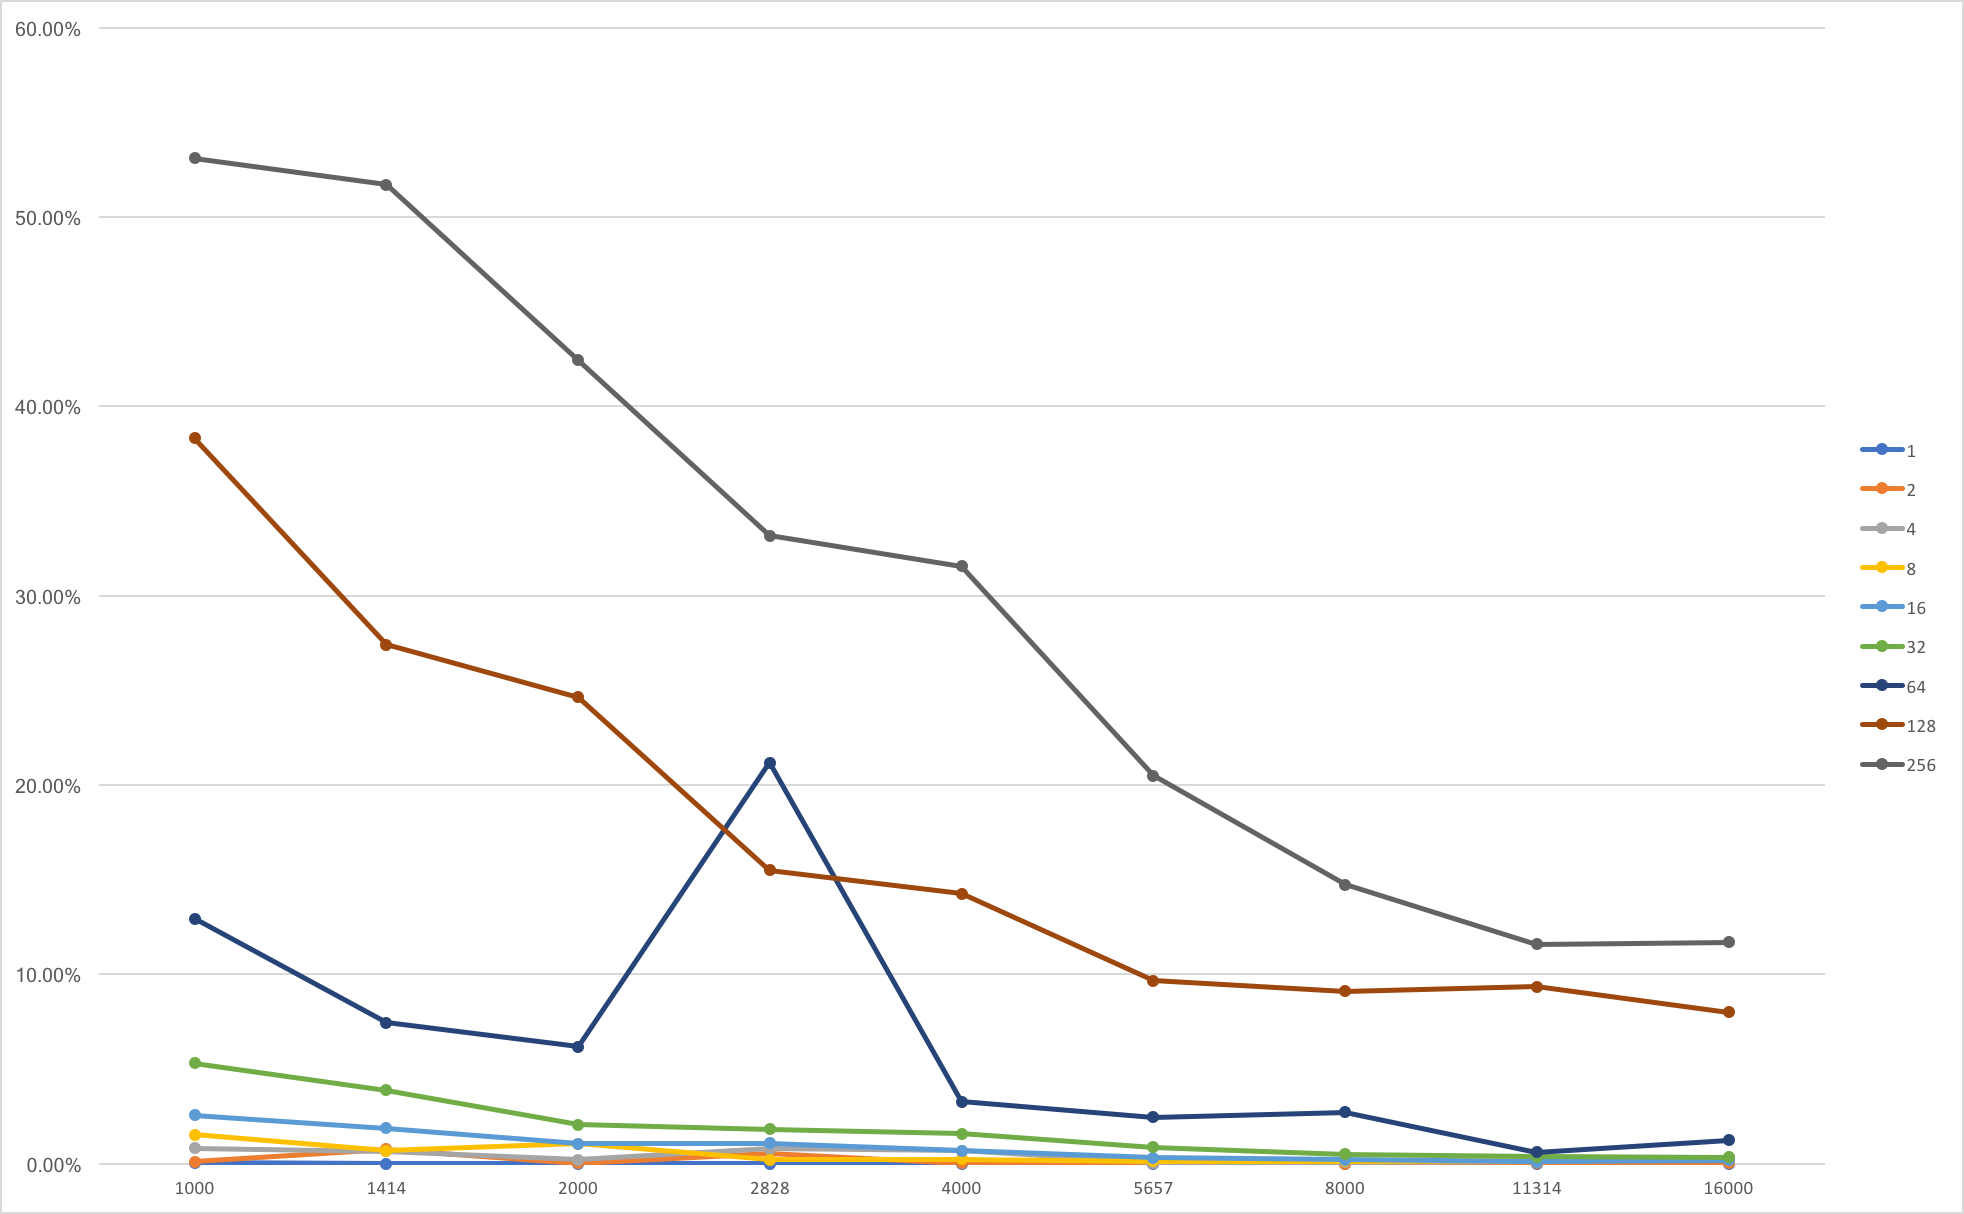
\includegraphics[width=\textwidth,keepaspectratio]{imgs/img07.png}
\end{figure}

\newpage

In figure.10 we can see here a similar behavior than in the strong scaling case, where the standard deviation increased as the number of particles increases proportionally to the number of ranks.

\begin{figure}[htb]
\caption{Time Standard Deviation - Ranks 2 to 16 }\label{fig:benchmark05}
\centering
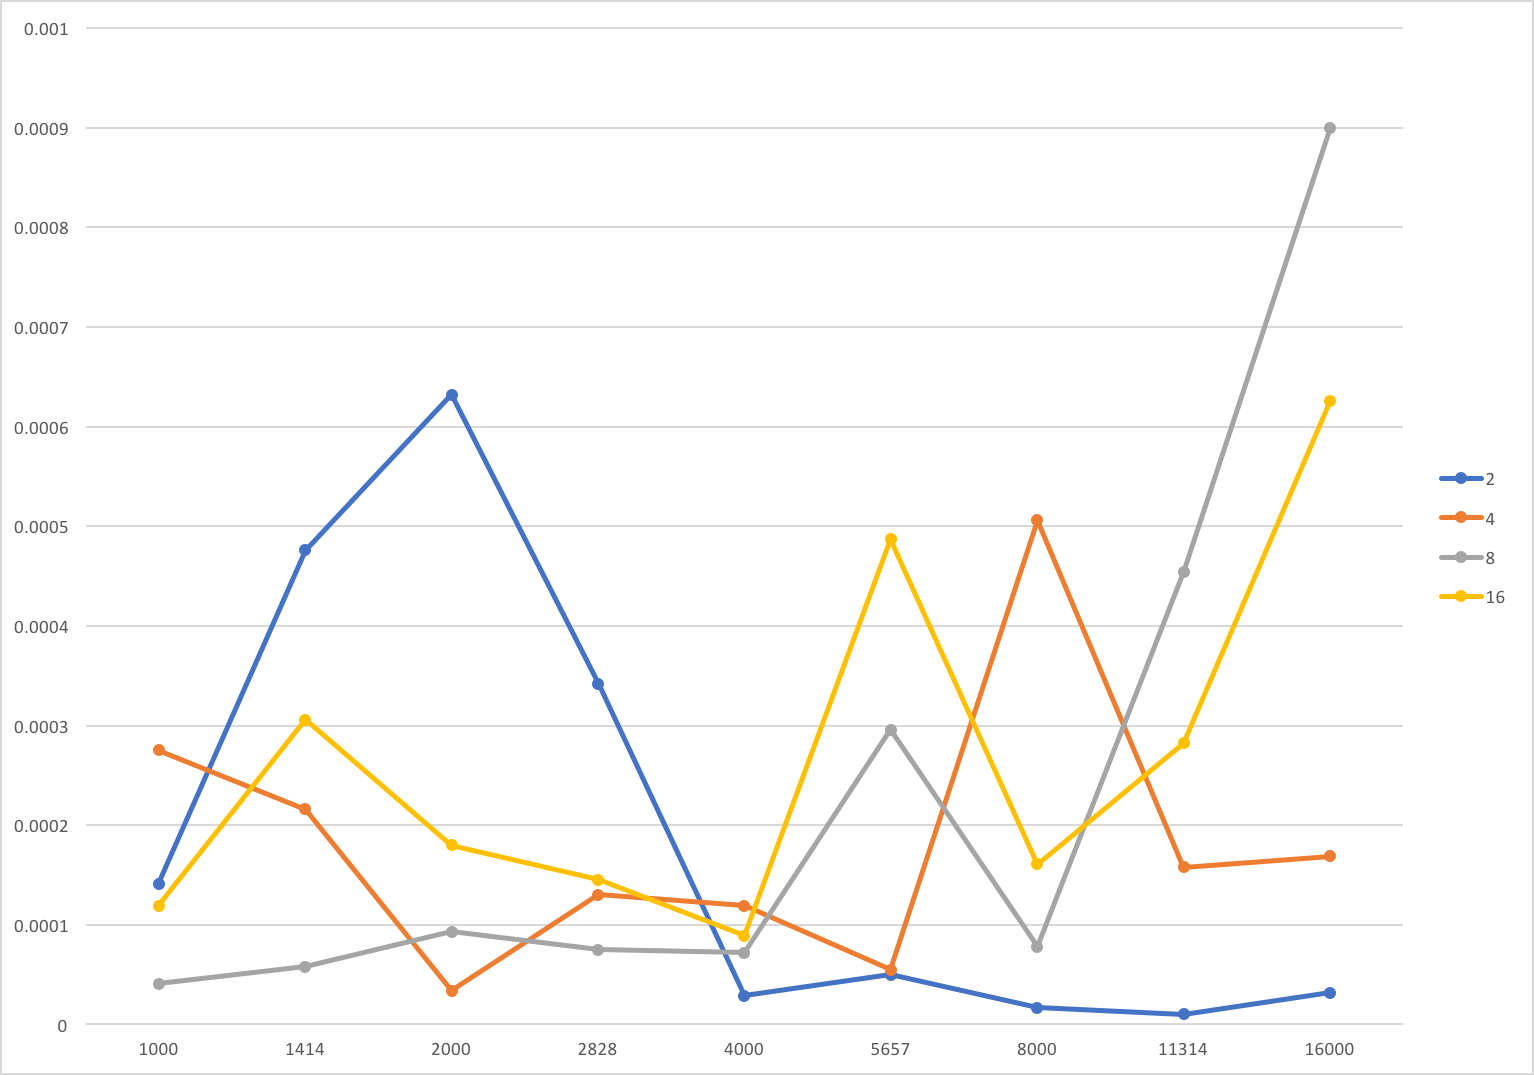
\includegraphics[width=\textwidth,keepaspectratio]{imgs/img010.png}
\end{figure}

\newpage

From figure.11 we can some spikes in the standard deviation but more or less the time spend in the MPI library for each rank are very close to each other. 

\begin{figure}[htb]
\caption{Time Standard Deviation - Ranks 32 to 256}\label{fig:benchmark05}
\centering
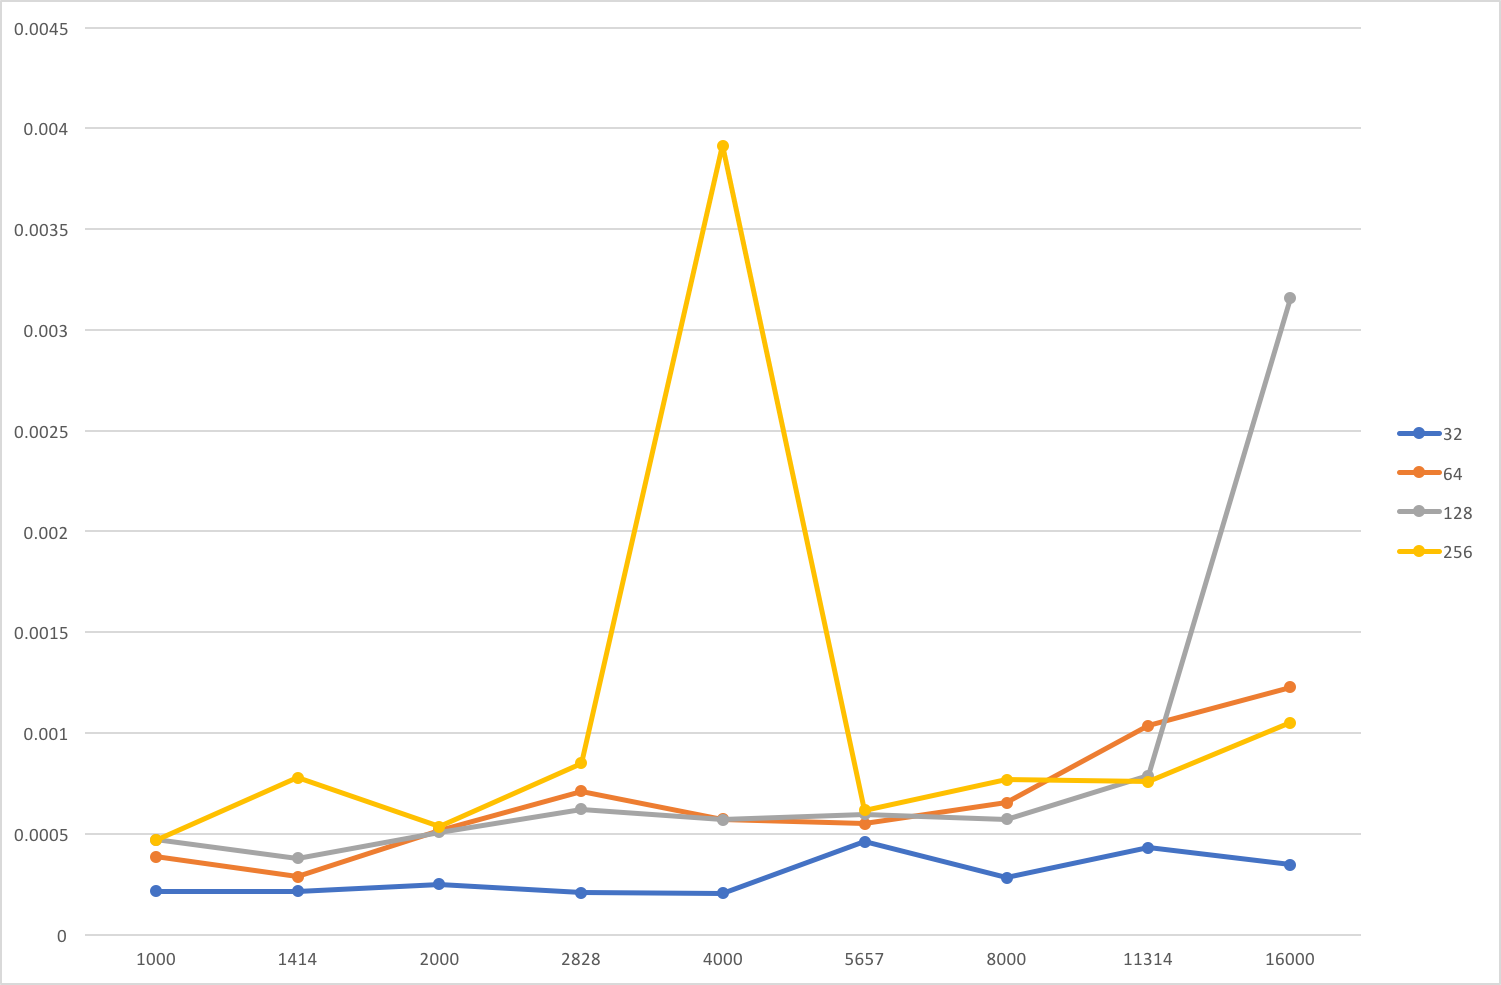
\includegraphics[width=\textwidth,keepaspectratio]{imgs/img011.png}
\end{figure}

\newpage


%----------------------------------------------------------------
%	SECTION 3 - REFERENCE
%----------------------------------------------------------------

\section{Reference}

\begin{flushleft}
Stampede2 User Guide -- Managing Memory \\ \url{https://portal.tacc.utexas.edu/user-guides/stampede2#managingmemory}

Introduction to High Performance Scientific Computing -- Victor Eijkhout \\ \url{http://pages.tacc.utexas.edu/~eijkhout/istc/istc.html}
\end{flushleft}

\begin{table}[htb]
\centering
\caption{Strong Scaling Benchmark - Number of Particles: 1000}
\resizebox{\textwidth}{!}{%
\begin{tabular}{@{}cccc@{}}
\toprule
\textbf{Threads} & \textbf{runtime-n1000} & \textbf{speed-up-n1000} & \textbf{efficiency-n1000} \\ \midrule
1	&	25.616771	&	1.00	&	1.00	\\
2	&	13.311931	&	1.92	&	0.96	\\
4	&	6.694731	&	3.83	&	0.96	\\
8	&	3.383455	&	7.57	&	0.95	\\
16	&	1.731183	&	14.80	&	0.92	\\
32	&	0.921504	&	27.80	&	0.87	\\
64	&	0.55232	&	46.38	&	0.72	\\
128	&	0.52906	&	48.42	&	0.38	\\
256	&	0.475464	&	53.88	&	0.21	\\  \bottomrule
\end{tabular}%
}
\end{table}

\begin{table}[]
\centering
\caption{Strong Scaling Benchmark - Number of Particles: 2000}
\resizebox{\textwidth}{!}{%
\begin{tabular}{@{}cccc@{}}
\toprule
\textbf{Threads} & \textbf{runtime-n2000} & \textbf{speed-up-n2000} & \textbf{efficiency-n2000} \\ \midrule
1	&	102.686432	&	1.00	&	1.00	\\
2	&	52.751255	&	1.95	&	0.97	\\
4	&	26.603915	&	3.86	&	0.96	\\
8	&	13.37015	&	7.68	&	0.96	\\
16	&	6.743617	&	15.23	&	0.95	\\
32	&	3.447329	&	29.79	&	0.93	\\
64	&	1.855324	&	55.35	&	0.86	\\
128	&	1.314569	&	78.11	&	0.61	\\
256	&	0.987171	&	104.02	&	0.41	\\  \bottomrule
\end{tabular}%
}
\end{table}

\begin{table}[]
\centering
\caption{Strong Scaling Benchmark - Number of Particles: 4000}
\resizebox{\textwidth}{!}{%
\begin{tabular}{@{}cccc@{}}
\toprule
\textbf{Threads} & \textbf{runtime-n4000} & \textbf{speed-up-n4000} & \textbf{efficiency-n4000} \\ \midrule
1	&	401.083066	&	1.00	&	1.00	\\
2	&	211.983822	&	1.89	&	0.95	\\
4	&	106.234969	&	3.78	&	0.94	\\
8	&	53.253804	&	7.53	&	0.94	\\
16	&	26.742206	&	15.00	&	0.94	\\
32	&	13.549024	&	29.60	&	0.93	\\
64	&	7.284818	&	55.06	&	0.86	\\
128	&	4.392116	&	91.32	&	0.71	\\
256	&	2.689669	&	149.12	&	0.58	\\  \bottomrule
\end{tabular}%
}
\end{table}

\begin{table}[]
\centering
\caption{Strong Scaling Benchmark - Number of Particles: 8000}
\resizebox{\textwidth}{!}{%
\begin{tabular}{@{}cccc@{}}
\toprule
\textbf{Threads} & \textbf{runtime-n8000} & \textbf{speed-up-n8000} & \textbf{efficiency-n8000} \\ \midrule
1	&	1605.582882	&	1.00	&	1.00	\\
2	&	848.64703	&	1.89	&	0.95	\\
4	&	423.841574	&	3.79	&	0.95	\\
8	&	212.0057	&	7.57	&	0.95	\\
16	&	106.230821	&	15.11	&	0.94	\\
32	&	53.425171	&	30.05	&	0.94	\\
64	&	27.256258	&	58.91	&	0.92	\\
128	&	15.092496	&	106.38	&	0.83	\\
256	&	8.370041	&	191.82	&	0.75	\\  \bottomrule
\end{tabular}%
}
\end{table}


\begin{table}[]
\centering
\caption{Strong Scaling Benchmark - Number of Particles: 16000}
\resizebox{\textwidth}{!}{%
\begin{tabular}{@{}cccc@{}}
\toprule
\textbf{Threads} & \textbf{runtime-n8000} & \textbf{speed-up-n16000} & \textbf{efficiency-n16000} \\ \midrule
1	&	6377.472625	&	1.00	&	1.00	\\
2	&	3378.441181	&	1.89	&	0.94	\\
4	&	1696.065717	&	3.76	&	0.94	\\
8	&	847.309032	&	7.53	&	0.94	\\
16	&	424.780338	&	15.01	&	0.94	\\
32	&	212.832976	&	29.96	&	0.94	\\
64	&	122.983181	&	51.86	&	0.81	\\
128	&	60.241818	&	105.86	&	0.83	\\
256	&	32.099958	&	198.68	&	0.78	\\  \bottomrule
\end{tabular}%
}
\end{table}


\begin{table}[]
\centering
\caption{Weak Scaling  Benchmark (n particles) - Efficiency Table }
\resizebox{\textwidth}{!}{%
\begin{tabular}{@{}cccccccccc@{}}
\toprule
\textbf{Threads}	&	\textbf{1000}&\textbf{1414}&\textbf{2000}&\textbf{2828}&\textbf{4000}&\textbf{5657}&\textbf{8000}&\textbf{11314}&\textbf{16000} 	\\ \midrule
1	&	100.0000\%	&		&		&		&		&		&		&		&		\\
2	&		&	96.1312\%	&		&		&		&		&		&		&		\\
4	&		&		&	95.7084\%	&		&		&		&		&		&		\\
8	&		&		&		&	95.9292\%	&		&		&		&		&		\\
16	&		&		&		&		&	95.6329\%	&		&		&		&		\\
32	&		&		&		&		&		&	95.1111\%	&		&		&		\\
64	&		&		&		&		&		&		&	93.1623\%	&		&		\\
128	&		&		&		&		&		&		&		&	85.3067\%	&		\\
256	&		&		&		&		&		&		&		&		&	80.4174\%	\\  \bottomrule
\end{tabular}%
}
\end{table}


\begin{table}[]										
\centering										
\caption{Weak Scaling - Average Runtime}										
\resizebox{\textwidth}{!}{%										
\begin{tabular}{@{}cccccccccc@{}}										
\toprule										
\textbf{Threads}	&	\textbf{runtime-n1000}&\textbf{runtime-n1414}&\textbf{runtime-n2000}&\textbf{runtime-n2828}	\\ \midrule							
1	&	25.57	&	51.15	&	101.93	&	201.88	\\	
2	&	13.29	&	26.6	&	53.07	&	105.99	\\	
4	&	6.71	&	13.32	&	26.72	&	53.14	\\	
8	&	3.37	&	6.72	&	13.35	&	26.66	\\	
16	&	1.74	&	3.42	&	6.74	&	13.4	\\	
32	&	0.93	&	1.78	&	3.44	&	6.8	\\	
64	&	0.54	&	0.99	&	1.87	&	4.51	\\	
128	&	0.51	&	0.74	&	1.3	&	2.22	\\	
256	&	0.48	&	0.62	&	0.91	&	1.53	\\  \bottomrule	
\end{tabular}%										
}										
\end{table}										

\begin{table}[]											
\centering											
\caption{Weak Scaling - Average Runtime}											
\resizebox{\textwidth}{!}{%											
\begin{tabular}{@{}cccccc@{}}											
\toprule											
\textbf{Threads}	&	\textbf{runtime-n4000}&\textbf{runtime-n5657}&\textbf{runtime-n8000}&\textbf{runtime-n11314}&\textbf{runtime-n16000} 	\\ \midrule								
1	&	407.63	&	813.53	&	1601.81	&	3193.35	&	6405.9	\\
2	&	210.55	&	424.36	&	847.92	&	1690.81	&	3380.19	\\
4	&	106.13	&	212.42	&	423.99	&	851.26	&	1693.11	\\
8	&	53.16	&	106.27	&	211.97	&	424.2	&	847.38	\\
16	&	26.74	&	53.34	&	106.17	&	212.61	&	423.71	\\
32	&	13.56	&	26.89	&	53.41	&	106.8	&	213.07	\\
64	&	7.01	&	13.81	&	27.45	&	57.97	&	110.31	\\
128	&	4.19	&	7.69	&	14.99	&	29.98	&	59.42	\\
256	&	2.74	&	4.59	&	8.2	&	15.64	&	31.8	\\  \bottomrule
\end{tabular}%											
}											
\end{table}											

\newpage
										
\begin{figure}[]
\caption{OpenMPI - Update and Search Functions}\label{fig:benchmark01}
\begin{lstlisting}
void search (ValueType pos[], ValueType vel[], ValueType mass[], 
ValueType acc[], const int n)
{
    
    int myRank, numProcs;
    callMPI( MPI_Comm_size(MPI_COMM_WORLD,&numProcs) );
    callMPI( MPI_Comm_rank(MPI_COMM_WORLD,&myRank)   );
    int partition_start, partition_end;
    partition_range( 0, n, numProcs, myRank, partition_start, partition_end );
    ValueType minv = 1e10, maxv = 0, ave = 0;
    
    for (int i = partition_start; i < partition_end; ++i)
    {
        ValueType vmag = 0;
        for (int k = 0; k < NDIM; ++k)
            vmag += (vel[ index(i,k) ] * vel[ index(i,k) ] );
        
        vmag = sqrt(vmag);
        maxv = std::max(maxv, vmag);
        minv = std::min(minv, vmag);
        ave += vmag;
    }
    
    ValueType g_maxv;
    callMPI(MPI_Reduce(&maxv, &g_maxv, 1, MPI_VALUE_TYPE, MPI_MAX, ROOT, MPI_COMM_WORLD));
    ValueType g_minv;
    callMPI(MPI_Reduce(&minv, &g_minv, 1, MPI_VALUE_TYPE, MPI_MIN, ROOT, MPI_COMM_WORLD));
    ValueType g_ave;
    callMPI(MPI_Reduce(&ave, &g_ave, 1, MPI_VALUE_TYPE, MPI_SUM, ROOT, MPI_COMM_WORLD));
    
    if (myRank==ROOT) {
        printf("min/max/ave velocity = %e, %e, %e\n", g_minv, g_maxv, g_ave/n);
    }
    callMPI(MPI_Barrier(MPI_COMM_WORLD));
}
\end{lstlisting}
\end{figure}

\begin{figure}[]
\caption{OpenMPI - Calculate Time}\label{fig:benchmark01}
\begin{lstlisting}
int main (int argc, char* argv[]) {
    ...
    callMPI(MPI_Bcast(pos, n*3, MPI_VALUE_TYPE, ROOT, MPI_COMM_WORLD));
    callMPI(MPI_Bcast(vel, n*3, MPI_VALUE_TYPE, ROOT, MPI_COMM_WORLD));
    callMPI(MPI_Bcast(mass, n, MPI_VALUE_TYPE, ROOT, MPI_COMM_WORLD));
    callMPI(MPI_Bcast(acc, n*3, MPI_VALUE_TYPE, ROOT, MPI_COMM_WORLD));
    myTimer_t t_start = getTimeStamp();
    double t_accel = 0, t_update = 0, t_search = 0, t_mpi;
    int flnum = 0;
    for (int step = 0; step < num_steps; ++step)
    {
        /* 1. Compute the acceleration on each object. */
        myTimer_t t0 = getTimeStamp();
        accel( pos, vel, mass, acc, n);
        myTimer_t t1 = getTimeStamp();
        /* 2. Advance the position and velocities. */
        update( pos, vel, mass, acc, n, dt);
        myTimer_t t2 = getTimeStamp();
        /* 3. Find the faster moving object. */
        if (step % 10 == 0)
            search( pos, vel, mass, acc, n);
        myTimer_t t3 = getTimeStamp();
        std::vector<int> counts(numProcs);
        std::vector<int> displ(numProcs);
        int partition_ranges;
        for (int i=0; i<numProcs; i++) {
            int pstart, pend;
            partition_range( 0, n, numProcs, i, pstart, pend );
            counts[i]=(pend-pstart)*3;
        }
        displ[0] = 0;
        for (int i = 1; i < numProcs; ++i)
            displ[i] = displ[i-1] + counts[i-1];
        callMPI(MPI_Allgatherv(MPI_IN_PLACE, 0, MPI_DATATYPE_NULL,
                                pos, &counts[0], &displ[0], MPI_VALUE_TYPE,
                                MPI_COMM_WORLD ));
        myTimer_t t4 = getTimeStamp();
        t_accel += getElapsedTime(t0,t1);
        t_update += getElapsedTime(t1,t2);
        t_search += getElapsedTime(t2,t3);
        t_mpi += getElapsedTime(t3,t4);
    }
}
\end{lstlisting}
\end{figure}

\begin{figure}[]
\caption{OpenMPI - Ranks Standard Deviation}\label{fig:benchmark01}
\begin{lstlisting}
int main (int argc, char* argv[]) {
	...
    double t_calc = getElapsedTime( t_start, getTimeStamp());
    
    float nkbytes = (float)((size_t)7 * sizeof(ValueType) * (size_t)n) / 1024.0f;
    
    /* variables used to calculate time standard deviation */
    double world_avg;
    double world_diff;
    double world_sd;
    double rank_avg,sum_difference;
    
    /* compute time standard deviation */
    rank_avg = t_calc*1000.0/num_steps;
    callMPI(MPI_Reduce(&rank_avg, &world_avg, 1, MPI_DOUBLE, MPI_SUM,ROOT,MPI_COMM_WORLD));
    world_avg = world_avg/numProcs;
    callMPI(MPI_Bcast(&world_avg, 1, MPI_DOUBLE, ROOT, MPI_COMM_WORLD));
    
    sum_difference = (rank_avg - world_avg)*(rank_avg - world_avg);
    callMPI(MPI_Reduce(&sum_difference, &world_diff, 1, MPI_DOUBLE, MPI_SUM,ROOT,MPI_COMM_WORLD));
    world_sd = sqrt(world_diff/numProcs);
    
    
    if (myRank==ROOT) {
        printf("Root[%d]: Average time = %f (ms) per step with %d elements, %.2f KB over %d steps\n", myRank, t_calc*1000.0/num_steps, n, nkbytes, num_steps);
        printf("Root[%d]: accel-time[%f] update-time[%f] search-time[%f] mpi-time[%f]\n", myRank,t_accel*1000/num_steps, t_update*1000/num_steps, t_search*1000/num_steps, t_mpi*1000/num_steps);
        printf("Total Ranks[%d] Standard Deviation: %f\n",numProcs,world_sd);
	}
}
\end{lstlisting}
\end{figure}

\begin{table}[]
\centering
\caption{Stampede2 - Compute Node (knl) - System Information}
\resizebox{\textwidth}{!}{%
\begin{tabular}{@{}ll@{}}
\toprule
\textbf{Architecture} & x86\_64 \\ \midrule
\textbf{CPU op-mode(s)} & 32-bit, 64-bit \\
\textbf{Byte Order} & Little Endian \\
\textbf{CPU(s)} & 272 \\
\textbf{On-line CPU(s) list} & 0-271 \\
\textbf{Thread(s) per core} & 4 \\
\textbf{Core(s) per socket} & 68 \\
\textbf{Socket(s)} & 1 \\
\textbf{NUMA node(s)} & 2 \\
\textbf{Vendor ID} & GenuineIntel \\
\textbf{CPU family} & 6 \\
\textbf{Model} & 87 \\
\textbf{Model name} & Intel(R) Xeon Phi(TM) CPU 7250 @ 1.40GHz \\
\textbf{Stepping} & 1 \\
\textbf{CPU MHz} & 1255.132 \\
\textbf{BogoMIPS} & 2793.44 \\
\textbf{L1d cache} & 32K \\
\textbf{L1i cache} & 32K \\
\textbf{L2 cache} & 1024K \\
\textbf{NUMA node0 CPU(s)} & 0-271 \\
\textbf{NUMA node1 CPU(s)} &  \\ \bottomrule
\end{tabular}%
}
\end{table}


\end{document}